\section{Introdução}

A Era da informação, com o advento da Internet (Web 2.0), está terminando. Estamos entrando na
Era da computação voltada ao consumidor, chamada por Grossman de \textit{Device Era}
\citep{grossman2012structure} e por Wirfs-Brock de 
\emph{Ambient Computing Era} \citep{wirfsbrock2011blog} (Figura \ref{fig:ambientcomputing_era}). 
Nesta era, focada no indivíduo, as pessoas possuem um ambiente rico em recursos e comunicação, 
principalmente através de dispositivos móveis. A computação é somente um alicerce para a entrega 
e melhoria de vida do indivíduo, o principal objetivo.

\begin{figure}[h]
        \centering
        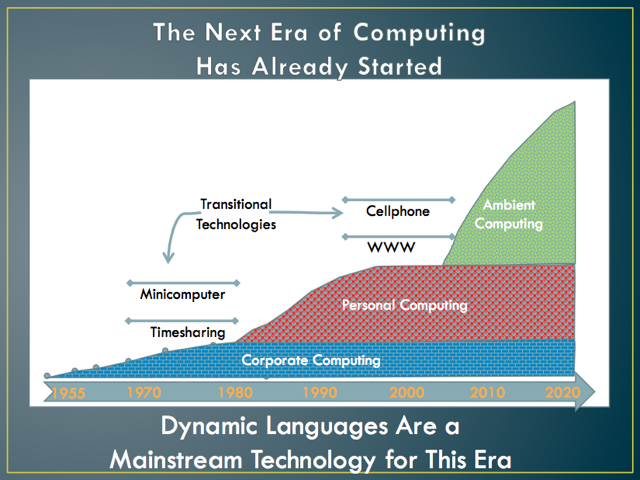
\includegraphics[width=0.7\linewidth]{3eras-medium.png}
        \caption{Eras da computação. Retirado do blog de Wirfs-Brock \citep{wirfsbrock2011blog}.}
        \label{fig:ambientcomputing_era}
\end{figure}


O que está acontecendo neste momento é que a quantidade de informação que se está gerando 
está em crescimento explosivo. Tecnologias consideradas de \emph{big data} tornam-se 
necessárias para se poder eficientemente armazenar, gerenciar, processar ou
visualizar essa quantidade massiva de informação. Talvez não na mesma velocidade, mas 
também com um extraordinário crescimento, novas tecnologias têm surgido para suprir tal
necessidade.

Este minicurso pretende explorar e diferenciar de forma introdutória diversas tecnologias recentes
para gerenciamento de dados na era do big data. Será utilizado como pano de fundo para os
exemplos um problema clássico da comunidade de bancos de dados: a contagem de triângulos.
Esta problema é perfeito para explicar as diferenças entre as tecnologias em termos de
expressividade e desempenho, pois pode ser representado por uma simples consulta SQL com
duas junções, contudo extremamente complexa de ser executada eficientemente. A partir deste
problema, podemos identificar como cada tecnologia se comporta em representar sua solução,
bem como seu desempenho. 

O minicurso está subdividido por tecnologia e na Seção \ref{sec:final} tecemos considerações finais
sobre o que ainda há de tecnologia a ser detalhada que não o fizemos aqui. A Seção \ref{sec:triangulos}
detalha o problema da contagem de triângulos, que irá permear as próximas seções de tecnologia. A Seção 
\ref{sec:relacional} mostra como funcionam bancos de dados relacionais tradicionais. As Seções 
\ref{sec:colunar} e \ref{sec:memoria} mostram as abordagens de bancos de dados orientados a colunas e 
em memória, respectivamente. A Seção \ref{sec:mpp} apresenta bancos de dados paralelos e introduz os 
conceitos de paralelismo de dados e computação para a Seção \ref{sec:hadoop} que apresenta o Hadoop e
alguns dos seus principais frameworks para análise de dados.

